\documentclass[10pt, aspectratio=169, handout]{beamer}
\usefonttheme{professionalfonts}

\mode<presentation>
{
  \usetheme{Berkeley}
  \usecolortheme{beaver}
  \usefonttheme{default}
  \setbeamertemplate{navigation symbols}{}
  \setbeamertemplate{caption}[numbered]
} 

\setbeamertemplate{footline}{%
  \leavevmode%
  \hbox{%
    \begin{beamercolorbox}[wd=.85\paperwidth,ht=2.5ex,dp=1ex,left]{author in head/foot}%
      \usebeamerfont{author in head/foot}Maxx Seminario, Electronic Circuits, Fall 2025%
    \end{beamercolorbox}%
    \begin{beamercolorbox}[wd=.15\paperwidth,ht=2.5ex,dp=1ex,right]{date in head/foot}%
      \hspace*{0.5em}\insertframenumber{} / \inserttotalframenumber\hspace*{0.5em}%
    \end{beamercolorbox}%
  }%
  \vskip0pt%
}

\usepackage[english]{babel}
\usepackage[utf8x]{inputenc}
\usepackage{tikz}
\usepackage{pgfplots}
\usepackage{array}
\usepackage{makecell}
\usepackage{verbatim}
\usepackage{graphicx}
\usepackage{subcaption}
\usepackage{amsfonts}
\usepackage{amsmath}
\usepackage{bm}
\usepackage{epstopdf}
\usepackage{circuitikz}
\usepackage{caption}
\captionsetup{compatibility=false}
\usepackage[absolute,overlay]{textpos}
\usetikzlibrary{calc}
\usetikzlibrary{pgfplots.fillbetween, backgrounds}
\usetikzlibrary{positioning}
\usetikzlibrary{pgfplots.groupplots}
\usetikzlibrary{plotmarks}
\usetikzlibrary{calc}
\usetikzlibrary{decorations.markings}
\usetikzlibrary{arrows.meta}

\usepgfplotslibrary{groupplots}
\pgfplotsset{compat=newest} 

\usepackage{hyperref}
\hypersetup{
    colorlinks=true,
    linkcolor=blue,
    filecolor=magenta,      
    urlcolor=cyan,
}

\title[ECEN 222]{Maxwell's Equations to Passive Circuit Elements}
\author{Maxx Seminario}
\institute{University of Nebraska-Lincoln}

\begin{document}
\begin{frame}
  \titlepage
\end{frame}

\section{Maxwell's Equations Review}

\begin{frame}{Maxwell's Equations: The Foundation}
    \textbf{There are four equations governing all electromagnetics}:

    \vspace{0.3cm}

    \renewcommand{\arraystretch}{1.4}
    \small
    \begin{tabular}{p{0.25\textwidth} p{0.33\textwidth} p{0.33\textwidth}}
        \textbf{Name} & \textbf{Integral Form} & \textbf{Differential Form} \\
        \hline
        Gauss's Law - Electric
        & $\displaystyle \oint_S \mathbf{E} \cdot d\mathbf{A} = \frac{Q_{\text{enc}}}{\epsilon_0}$ 
        & $\displaystyle \nabla \cdot \mathbf{E} = \frac{\rho}{\epsilon_0}$ \\[0.3cm]

        No magnetic monopoles
        & $\displaystyle \oint_S \mathbf{B} \cdot d\mathbf{A} = 0$
        & $\displaystyle \nabla \cdot \mathbf{B} = 0$ \\[0.3cm]

        Faraday's Law 
        & $\displaystyle \oint_C \mathbf{E} \cdot d\mathbf{l} = -\frac{d\Phi_B}{dt}$
        & $\displaystyle \nabla \times \mathbf{E} = -\frac{\partial \mathbf{B}}{\partial t}$ \\[0.3cm]

        Ampère-Maxwell Law 
        & $\displaystyle \oint_C \mathbf{B} \cdot d\mathbf{l} = \mu_0 I_{\text{enc}} + \mu_0 \epsilon_0 \frac{d\Phi_E}{dt}$
        & $\displaystyle \nabla \times \mathbf{B} = \mu_0 \mathbf{J} + \mu_0 \epsilon_0 \frac{\partial \mathbf{E}}{\partial t}$ \\
    \end{tabular}
\end{frame}

\begin{frame}{What Do Maxwell's Equations Tell Us?}
    
    \begin{columns}[t]
    \column{0.48\textwidth}
        \textbf{Gauss's Law}:
        \begin{itemize}
            \item Electric charges create electric fields
            \item Electric field lines start/end on charges
            \item Basis for \textbf{capacitance}
        \end{itemize}
        
        \vspace{0.5cm}
        
        \textbf{No Magnetic Monopoles}:
        \begin{itemize}
            \item Magnetic field lines form closed loops
            \item No isolated magnetic charges
            \item Magnetic fields from currents only
        \end{itemize}
        
    \column{0.48\textwidth}
        \textbf{Faraday's Law}:
        \begin{itemize}
            \item Changing magnetic flux creates voltage
            \item Basis for \textbf{inductance}
            \item Transformers, generators, motors
        \end{itemize}
        
        \vspace{0.5cm}
        
        \textbf{Ampère-Maxwell Law}:
        \begin{itemize}
            \item Currents create magnetic fields
            \item Changing electric fields create magnetic fields
            \item Basis for electromagnetic waves
        \end{itemize}
        
    \end{columns}
    
    \vspace{0.5cm}
    
    \begin{block}{For Circuit Theory}
        We focus on Gauss's Law (capacitors) and Faraday's Law (inductors)
    \end{block}
    
\end{frame}

\section{From Maxwell to Circuit Elements}

\begin{frame}{The Resistor:  Ohm's Law}
    
    \begin{columns}[t]
    \column{0.48\textwidth}
        \textbf{From Electromagnetics}:
        
        \vspace{0.2cm}
        
        Current density related to electric field:
        \[
        \bm{J} = \sigma \bm{E}
        \]
        
        where $\sigma$ is conductivity. 
        
        \vspace{0.3cm}
        
        Integrating over a conductor:
        \[
        I = \int_A \bm{J} \cdot d\bm{A}, \quad V = \int_l \bm{E} \cdot d\bm{l}
        \]
        
        \begin{block}{Leads to Ohm's Law} 
            $V = IR$, where $R = \dfrac{l}{\sigma A}$
        \end{block}
        
    \column{0.48\textwidth}
        \textbf{Circuit Symbol}:
        
        \vspace{0.5cm}
        
        \begin{figure}[htb]
        \centering
        \begin{circuitikz}[scale=1.3]
            % Resistor with current arrow
            \draw (0,0) to[R, l=$R$, i>=$I$] (3,0);

            % Voltage polarity markers
            \draw (1.1,0.8) node {$+$};
            \draw (1.9,0.8) node {$-$};

            % Voltage label between the polarity markers
            \draw (1.5,0.8) node {$V_R$};
        \end{circuitikz}
        \end{figure} 
        
        \vspace{0.5cm}
        
        \begin{block}{Power Dissipated:} 
        \[
        P = VI = I^2R = \frac{V^2}{R}
        \]
        \end{block}
        
        
    \end{columns}
    
\end{frame}

\begin{frame}{The Capacitor: Stored Electric Energy}
    
    \begin{columns}[t]
    \column{0.48\textwidth}
        \textbf{From Gauss's Law}:
        
        \vspace{0.2cm}
        
        Parallel plate capacitor:
        
        \begin{figure}[htb]
        \centering
        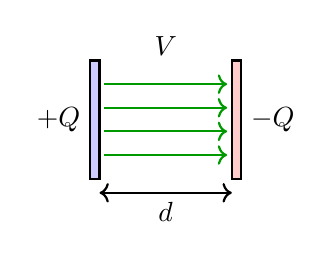
\begin{tikzpicture}[scale=0.6]
            % Left plate
            \draw[fill=blue! 20, thick] (0,0) rectangle (0.2,2.5);
            \node[left] at (0,1.25) {$+Q$};
            
            % Right plate
            \draw[fill=red!20, thick] (3,0) rectangle (3.2,2.5);
            \node[right] at (3.2,1.25) {$-Q$};
            
            % Electric field lines
            \foreach \y in {0.5, 1.0, 1.5, 2.0}
                \draw[->, thick, green! 60! black] (0.3,\y) -- (2.9,\y);
            
            % Distance label
            \draw[<->, thick] (0.2,-0.3) -- (3,-0.3);
            \node[below] at (1.6,-0.3) {$d$};
            
            % Voltage label
            \node at (1.6,2.8) {$V$};
        \end{tikzpicture}
        \end{figure}
        
        Electric field:  $E = \frac{Q}{\epsilon_0 A}$
        
        \vspace{0.1cm}

        Voltage: $V = Ed = \frac{Qd}{\epsilon_0 A}$
        
        \[
        Q = CV \quad \text{where} \quad C = \frac{\epsilon_0 A}{d}
        \]
        
    \column{0.48\textwidth}
        \textbf{Circuit Symbol}:
        
        \begin{figure}[htb]
        \centering
        \begin{circuitikz}[scale=1.0]
            % Capacitor with current arrow
            \draw (0,0) to[C, l=$C$, i>=$I$] (3,0);

            % Voltage polarity markers
            \draw (1.1,1.2) node {$+$};
            \draw (1.9,1.2) node {$-$};

            % Voltage label
            \draw (1.5,1.2) node {$V$};
        \end{circuitikz}
        \end{figure}
        

        \begin{block}{I-V Relationship}
            $I = C\frac{dV}{dt}$      
        \end{block}


        \begin{block}{Stored Energy:}
            \begin{itemize}
                \item $W = \frac{1}{2}CV^2 = \frac{1}{2}QV$
                \item Stores energy in electric field
            \end{itemize}
        \end{block}
    \end{columns}
    
\end{frame}

\begin{frame}{The Inductor: Stored Magnetic Energy}
    
    \begin{columns}[t]
    \column{0.48\textwidth}
        \textbf{From Faraday's Law}:
        
        Solenoid inductor:
        
        \begin{figure}[htb]
        \centering
        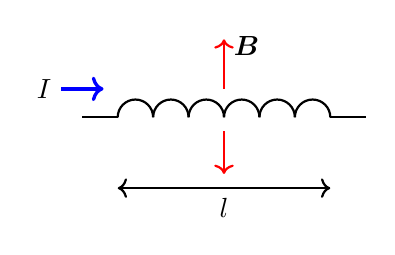
\begin{tikzpicture}[scale=0.9]
            % Leads
            \draw[thick] (-0.5,0) -- (0,0);
            \draw[thick] (3,0) -- (3.5,0);

            % Solenoid coil (nicely spaced loops)
            \foreach \x in {0,0.5,...,2.5} {
                \draw[thick] (\x,0) arc (180:0:0.25);
            }

            % Current arrow on the left lead
            \draw[->, very thick, blue] (-0.8,0.4) -- (-0.2,0.4);
            \node[left] at (-0.8,0.4) {$I$};

            % Magnetic field indication (inside core)
            \draw[->, thick, red] (1.5,0.4) -- (1.5,1.1);
            \draw[->, thick, red] (1.5,-0.2) -- (1.5,-0.8);
            \node[right] at (1.5,1) {$\bm{B}$};

            % Length label under coil
            \draw[<->, thick] (0,-1.0) -- (3,-1.0);
            \node[below] at (1.5,-1.0) {$l$};
        \end{tikzpicture}
        \end{figure}

        \vspace{0.4cm}
        
        Magnetic flux:  $\Phi_B = N B A$ 
        
        Faraday's Law: $V = -\dfrac{d\Phi_B}{dt}$
        
        For $B = \dfrac{\mu_0 N I}{l}$:
        
        % \[
        % V = L\frac{dI}{dt} \quad \text{where} \quad L = \frac{\mu_0 N^2 A}{l}
        % \]
        
    \column{0.48\textwidth}
        \textbf{Circuit Symbol}:
        
        \begin{figure}[htb]
        \centering
        \begin{circuitikz}[scale=1.2]
            % Inductor with current arrow
            \draw (0,0) to[L, l=$L$, i>=$I$] (3,0);

            % Voltage polarity markers
            \draw (1.1,0.8) node {$+$};
            \draw (1.9,0.8) node {$-$};

            % Voltage label
            \draw (1.5,0.8) node {$V$};
        \end{circuitikz}
        \end{figure}

        \begin{block}{I-V Relationship:}
            $V = L\frac{dI}{dt}$  
            where $L = \dfrac{\mu_0 N^2 A}{l}$
        \end{block}

        \begin{block}{Stored Energy:}
            \begin{itemize}
                \item $W = \frac{1}{2}LI^2$
                \item Stores energy in magnetic field
            \end{itemize}
        \end{block}
        
    \end{columns}
    
\end{frame}

\begin{frame}{Passives Summary}
    
    \begin{table}
    \centering
    \begin{tabular}{|c|c|c|c|}
    \hline
    \textbf{Element} & \textbf{Symbol} & \textbf{I-V Relation} & \textbf{Energy/Power} \\
    \hline
    \hline
    Resistor & \begin{circuitikz}\draw (0,0) to[R, l=$R$] (1.5,0);\end{circuitikz} & $V = IR$ & $P = I^2R$ (dissipated) \\
    \hline
    Capacitor & \begin{circuitikz}\draw (0,0) to[C, l=$C$] (1.5,0);\end{circuitikz} & $I = C\frac{dV}{dt}$ & $W = \frac{1}{2}CV^2$ (stored) \\
    \hline
    Inductor & \begin{circuitikz}\draw (0,0) to[L, l=$L$] (1.5,0);\end{circuitikz} & $V = L\frac{dI}{dt}$ & $W = \frac{1}{2}LI^2$ (stored) \\
    \hline
    \end{tabular}
    \end{table}
    
    \vspace{0.5cm}
    
    \begin{columns}[t]
    \column{0.32\textwidth}
        \textbf{Resistor (R)}:
        \begin{itemize}
            \item From $\bm{J} = \sigma\bm{E}$
            \item Dissipates energy
            \item Algebraic relation
        \end{itemize}
        
    \column{0.32\textwidth}
        \textbf{Capacitor (C)}:
        \begin{itemize}
            \item From Gauss's Law
            \item Stores electric energy
            \item Time derivative of $V$
        \end{itemize}
        
    \column{0.32\textwidth}
        \textbf{Inductor (L)}:
        \begin{itemize}
            \item From Faraday's Law
            \item Stores magnetic energy
            \item Time derivative of $I$
        \end{itemize}
        
    \end{columns}
    
    \vspace{0.5cm}
    
    \begin{block}{Connection to Maxwell}
        Circuit elements are macroscopic manifestations of Maxwell's equations! 
    \end{block}
    
\end{frame}

% \begin{frame}{Frequency Domain Behavior}
    
%     \textbf{Impedance}:  Generalization of resistance to AC circuits
    
%     \vspace{0.3cm}
    
%     For sinusoidal signals $v(t) = V_0 e^{j\omega t}$, $i(t) = I_0 e^{j\omega t}$:
    
%     \vspace{0.5cm}
    
%     \begin{table}
%     \centering
%     \begin{tabular}{|c|c|c|c|}
%     \hline
%     \textbf{Element} & \textbf{Impedance} & \textbf{Low Freq ($\omega \to 0$)} & \textbf{High Freq ($\omega \to \infty$)} \\
%     \hline
%     \hline
%     Resistor & $Z_R = R$ & $R$ & $R$ \\
%     \hline
%     Capacitor & $Z_C = \frac{1}{j\omega C}$ & Open circuit ($\infty$) & Short circuit ($0$) \\
%     \hline
%     Inductor & $Z_L = j\omega L$ & Short circuit ($0$) & Open circuit ($\infty$) \\
%     \hline
%     \end{tabular}
%     \end{table}
    
%     \vspace{0.5cm}
    
%     \begin{block}{Key Insight}
%         \begin{itemize}
%             \item \textbf{Capacitors}:  Block DC, pass AC (high-pass behavior)
%             \item \textbf{Inductors}: Pass DC, block AC (low-pass behavior)
%             \item \textbf{Resistors}: Frequency-independent
%         \end{itemize}
%     \end{block}
    
% \end{frame}

\section{Summary}

\begin{frame}{Summary}
    
    \begin{columns}[t]
    \column{0.48\textwidth}
        \textbf{Maxwell's Equations}:
        \begin{itemize}
            \item Four fundamental laws
            \item Gauss's Law $\rightarrow$ capacitors
            \item Faraday's Law $\rightarrow$ inductors
            \item Unified theory of E\&M
        \end{itemize}
        
        \vspace{0.5cm}
        
        \textbf{Circuit Elements IV Relations}: 
        \begin{itemize}
            \item \textbf{R}: Dissipates energy ($V = IR$)
            \item \textbf{C}:  Stores electric energy ($I = C\frac{dV}{dt}$)
            \item \textbf{L}: Stores magnetic energy ($V = L\frac{dI}{dt}$)
        \end{itemize}
        
    \column{0.48\textwidth}
        \textbf{Frequency Behavior}: 
        \begin{itemize}
            % \item Impedance: $Z(\omega)$
            \item Capacitors: block DC, pass AC
            \item Inductors: pass DC, block AC
            \item Resistors: frequency-independent
        \end{itemize}
        
        \vspace{0.5cm}
        
        \textbf{Energy Storage}:
        \begin{itemize}
            \item Capacitor: $W_C = \frac{1}{2}CV^2$
            \item Inductor: $W_L = \frac{1}{2}LI^2$
            \item Only R dissipates energy
        \end{itemize}
        
    \end{columns}
    
    \vspace{0.5cm}
    
    \begin{alertblock}{Big Picture}
        Passive circuit theory is the application of Maxwell's equations!
    \end{alertblock}
    
\end{frame}

\end{document}